% This file is part of the stream_information project.
% Copyright 2017 the authors. All rights reserved.

% TODO:
% - Reference for the dustmaps package? See software section.

% Story:
% - progenitor - show std_v, std_phi2
% - 2 gaps, 1 under-density - epicycles/streakline? percentiles in polynomial
% - spur - encounter?

% Make the point that if we can measure distance to spur, stream, RVs - measure energy offset which doesn't depend on time, like gap size

% Make sure to include simple equations so can rescale

% Note that epicyclic density variations naturally in, but caveat uniform release times

\documentclass[modern]{aastex62}

\usepackage{amsmath}

% typography
\setlength{\parindent}{1.\baselineskip}
\newcommand{\acronym}[1]{{\small{#1}}}
\newcommand{\package}[1]{\textsl{#1}}
\newcommand{\gaia}{\textsl{Gaia}}
\newcommand{\pans}{\textsl{Pan-STARRS}}
\newcommand{\DR}{\acronym{DR2}}
\newcommand{\msun}{\textrm{M}_\odot}
\newcommand{\kpc}{\textrm{kpc}}
% \newcommand{\mag}{\textrm{mag}}
\newcommand{\kms}{\ensuremath{\textrm{km}~\textrm{s}^{-1}}}
\newcommand{\bs}[1]{\boldsymbol{#1}}
\newcommand{\masyr}{\ensuremath{\textrm{mas}~\textrm{yr}^{-1}}}
\newcommand{\feh}{\ensuremath{[\textrm{Fe} / \textrm{H}]}}
\newcommand{\article}{\textsl{Letter}}

\newcommand{\sectionname}{Section}
\newcommand{\equationname}{Equation}
\renewcommand{\tablename}{Table}

\newcommand{\todo}[1]{{\color{red} TODO: #1}}

% aastex parameters
% \received{not yet; THIS IS A DRAFT}
%\revised{not yet}
%\accepted{not yet}
% % Adds "Submitted to " the arguement.
% \submitjournal{ApJ}
\shorttitle{GD-1 in Gaia DR2}
\shortauthors{Price-Whelan \& Bonaca}

%@arxiver{}

\begin{document}\sloppy\sloppypar\raggedbottom\frenchspacing % trust me

\title{Off the beaten path: \\
       Gaia reveals GD-1 stars perturbed off of the main stream track}
% Gaia DR2 reveals stream stars...
% A first look at the GD-1 stellar stream with Gaia DR2

\author[0000-0003-0872-7098]{Adrian~M.~Price-Whelan}
\altaffiliation{These authors contributed equally to this work.}
\affiliation{Department of Astrophysical Sciences,
             Princeton University, Princeton, NJ 08544, USA}
\email{adrn@astro.princeton.edu}
\correspondingauthor{Adrian M. Price-Whelan}

\author[0000-0002-7846-9787]{Ana Bonaca}
\altaffiliation{These authors contributed equally to this work.}
\affil{Harvard--Smithsonian Center for Astrophysics, Cambridge, MA 02138, USA}

\begin{abstract}\noindent % trust me
Tidally-disrupted globular clusters are transformed into thin, dynamically-cold
streams of stars that are extremely valuable tracers of the large- and
small-scale distribution of mass in the Galaxy.
Most stellar streams discovered around the Milky Way reside in the Galactic halo
and are therefore primarily sensitive to the dark matter distribution.
% The longest and most prominent thin stream in the Milky Way --- the GD-1 stream --- has been used
% to constrain the shape of the inner halo, and is a promising place to search for
% signatures of dark matter subhalo interactions.
Here we present a sample of highly-probable members of the longest cold stream, GD-1, selected to have
small parallaxes and retrograde proper motions using data from the \gaia\
mission, and \pans\ photometry consistent with an old and metal-poor population
at a distance of $\sim10~\kpc$.
This selection extends the stream by $20^\circ$, reveals a plausible location of
the progenitor, and shows significant density variations along the stream in
unprecedented detail.
In addition to confirming several prominent gaps detected in photometric maps of GD-1, for the first time we find evidence
of stream members off of the main track.
These features might be an indication of complex internal kinematics within a progenitor unlike any of the known globular clusters, or a result of a stream interaction with a massive perturber.
% Detailed modeling of the positional and velocity offsets
% or an indication of complex internal kinematics within the
% stream progenitor.
% Velocity offset between these features and the stream is an order of magnitude larger than the variance in velocity fields of known globular cluster, thus favoring the encounter origin.
% If this is confirmed, off-stream features will enable a robust estimate of the perturber's mass.
% If caused by a subhalo interaction, we estimate that the detected underdensity
% and the associated spur could have been induced by a perturbation of a
% $\sim10^7\,\rm M_\odot$(?) object $\sim 0.5\,$Gyr ago.
\end{abstract}

\keywords{Galaxy: halo --- dark matter}

\section{Introduction}
\label{sec:intro}

Dynamically cold stellar streams are formed during the tidal disruption of stellar
systems by the gravitational field of their host galaxy.
The phase-space density and mean track of stars in streams therefore encode
information about the underlying distribution and shape of mass on galactic
scales (e.g., \citealt{Johnston:1999, Bonaca:2018}).
% Most stellar streams are found in the halos of galaxies and are therefore
% important tracers of the large-scale distribution of dark matter in galactic
% halos.
% Long, thin stellar streams are also excellent laboratories for studying
% small-scale structures in the mass distribution:
% thin streams can remain coherent for tens of orbital periods, depending in
% detail on the symmetries of the underlying galactic mass distribution (e.g.,
% \citealt{Erkal:2016a}).
Being dynamically cold, stellar streams can retain any imprints on its phase-space density from encounters with a massive perturber for close to its total survival time \citep[e.g.,][]{Yoon:2011}.
% Encounters between massive perturbers and stream stars imprint variations in the
% phase-space density that can persist and remain visible for close to their total
% survival time (e.g., \citealt{Yoon:2011}).
In this sense, streams represent one of the most promising directions for
testing the existence of small-scale dark matter sub-halos, predicted by
standard $\Lambda$ Cold Dark Matter ($\Lambda$CDM) theory
(\citealt{Erkal:2015, Sanders:2016, Bovy:2017}).

Over 30 candidate stellar streams have been discovered in the Milky Way \citep[see][for a recent review]{Grillmair:2016, Newberg:2016}.
% thanks to large-area, multi-band photometric surveys (especially
% the Sloan Digital Sky Survey, SDSS; \citealt{York:2000}).
% The Milky Way streams have a wide range of properties such as length, velocity
% dispersion, and density (e.g., \citealt{Odenkirchen:2001, Grillmair:2006,
% Grillmair:2006b, Belokurov:2006, Belokurov:2007, Bonaca:2012, Shipp:2018}; see
% also the recent review \citealt{Grillmair:2016, Newberg:2016}).
% , and the majority
% have no obvious, bound progenitor systems;
% of the thin, likely globular-cluster-origin streams, only two have clear
% progenitors (NGC 5466 and Palomar 5).
% Most streams were first detected as a linear overdensity in stellar counts filtered to preferentially select faint blue stars, most likely members of a former Galactic satellite.
GD-1 is the most prominent among the thin streams, discovered as an arcing overdensity of faint blue stars in the SDSS photometry \citep{Grillmair:2006}.
It spans $\sim 60^\circ$ on the sky, which at its distance between $\sim 7$--$10~\textrm{kpc}$ translates to a physical length of $\sim 15~\kpc$.
No remnant progenitor has been associated with the stream, but its
width ($\sigma \approx 12'$), metallicity ($\feh \approx -1.4$), and estimated
stellar mass ($M \approx 2 \times 10^4~\msun$)
imply that GD-1 is a disrupted globular cluster \citep{Koposov:2010}.

Its length and location in the
Galactic halo (pericentric distance $r_\textrm{peri} \sim 13~\kpc$) make GD-1 an
ideal object for constraining the gravitational potential of dark matter in the
inner Milky Way.
Indeed, both from fitting orbits to binned phase-space measurements along the
GD-1 stream (\citealt{Koposov:2010}) and from modeling the stream track in
phase-space coordinates \citep{Bowden:2015, Bovy:2016}, we learned that the
dark matter distribution in the inner $\approx20\,\rm kpc$ is consistent with being close to
spherical.
This is in line with findings from simulated Milky Way-like galaxies; while dark matter halos are in general expected to be triaxial \citep{Allgood:2006}, the baryonic processes forming galaxies tend to make their inner regions more spherical \citep{Zhu:2016}.

An implied old dynamical age, combined with its orbital properties, makes GD-1 a prime stream to not only map the dark matter on large scales, but to also study its small scale structure.
Density variations in the stream can be induced from interactions with dark matter subhalos \citep[e.g.,][]{Ngan:2014}, but also from interactions with giant molecular clouds \citep{Amorisco:2016} or resonant encounters with the bar \citep{Pearson:2017}.
However, these baryonic effects are unlikely to have perturbed GD-1 because of its large pericentric distance and retrograde orbit with respect to
the Galactic bar.
By estimating a stream age of $\approx 4~\textrm{Gyr}$, assuming a progenitor
mass of $10^5~\msun$, and by assuming properties of the subhalo population from dark matter-only simulations \citep[scaled to the Milky Way halo mass of $10^{12}\,\msun$, and reduced in number by a factor of 3 to account for disruption by the Galactic disk]{Springel:2008, Diemand:2008}, \citet{Erkal:2016} predict that GD-1 could have up to one significant, wide
($\approx 5$--$7^\circ$) gap caused by an interaction with a
$10^6$--$10^7~\msun$ subhalo.
A definitive ruling on the presence of dark matter subhalos in this mass regime would directly inform on the nature of dark matter \citep[e.g.][]{Bullock:2017}.

Photometric studies of GD-1 revealed the presence of density variations and gaps along the stream, as well as wiggles in the main stream track \citep[][]{Carlberg:2013, DeBoer:2018}.
Purely photometric stream studies suffer to some extent from contamination of the Milky Way foreground, whose small-scale spatial variations could partially account for density inhomogeneities reported along cold streams \citep[e.g.,][]{Ibata:2016}.
In this \article, we improve upon the selection of likely GD-1 members by using astrometric data from the \gaia\ mission, in addition to precise photometry from the \pans\ survey (\S\,\ref{sec:data}).
This data enabled us to measure global properties of GD-1 to an unprecedented precision (\S\,\ref{sec:res_global}), and detect clear signatures of stream stars beyond the main track (\S\,\ref{sec:res_gap}).
Implications of this revolutionary remapping of GD-1 are discussed in \S\,\ref{sec:discussion}.
% \todo{hints of density variations} from initial work Koposov:2010, later confirmed by density modeling, but all low significance
% (\citealt{Carlberg:2013}).
% More recently, deep photometry of GD-1 from CFHT/Megacam has revealed
% interesting small-scale ``wiggles'' and significant density variations along a $\approx 45^\circ$ span of the stream (\citealt{DeBoer:2018}):
% [summarize their conclusions].
% \todo{these analyses relied on binned data, still contaminated by MW stars}
%
% In this \article, we present clearest view of the GD-1 stream to date using
% astrometric data from the \gaia\ mission data release 2 (\DR) combined with
% precise photometry from the \pans\ survey.
% We find XX under-densities gaps, some consistent with ...
% We revisit...do not try to model or fit for Galactic potential.
% Focus on stream properties, data.


\section{Data}
\label{sec:data}

We use astrometric data from the \gaia\ mission (\citealt{Prusti:2016}), data
release 2 (\citealt{Gaia-Collaboration:2018, Lindegren:2018}), and photometry
from the \pans\ survey, data release 1 (\citealt{Chambers:2016}) to select
high-confidence members of the GD-1 stream.

We retrieve \gaia\ data along the previously-identified track of the GD-1 stream
from the \gaia\ science archive\footnote{\url{https://gea.esac.esa.int/}} by
selecting all sources with small parallax, $\varpi < 1~\textrm{mas}$, and use a
set of spherical polygons to select batches of stars that have small latitude in
the heliocentric GD-1 coordinate system, $(\phi_1, \phi_2)$, defined in
\cite{Koposov:2010}.\footnote{This transformation is implemented using the
\package{Astropy} (\citealt{astropy}) coordinate transformation framework in the
\package{Gala} \texttt{Python} package (\citealt{gala}).}
We convert the sky coordinates and proper motions of the parallax-selected stars
to the GD-1 stream coordinate system, and correct the proper motions for solar
reflex motion by assuming that stars at a given stream longitude, $\phi_1$, have
a distance given by the linear relationship $d(\phi_1) = (0.05 \, \phi_1 +
10)~\textrm{kpc}$.
For the solar velocity in a Galactocentric rest frame, we use $\bs{v}_\odot =
(11.1, 232.24, 7.25)~\kms$ (\citealt{Schonrich:2010, Bovy:2015}).
\figurename~\ref{fig:selection} (top right) shows the distribution of stars with
$|\phi_2| < 1^\circ$ in solar-reflex-corrected proper motion components in the
GD-1 coordinate system, $\mu_{\phi_1, \odot}$ (which includes the $\cos{\phi_2}$
term) and $\mu_{\phi_2, \odot}$.
GD-1 member stars are visible as the over-density around
$(\mu_{\phi_1, \odot}, \mu_{\phi_2, \odot}) \approx (-8, 0)~\masyr$.

As a first selection of GD-1 candidate member stars, we select stars with proper
motions $-9 < \mu_{\phi_1, \odot} < -4.5~\masyr$ and $-1.7 < \mu_{\phi_2, \odot}
< 1~\masyr$, as visualized by the orange rectangle in the top right panel of
\figurename~\ref{fig:selection}.
\figurename~\ref{fig:selection} (top left) shows all stars the pass the
selection on proper motion, plotted in the GD-1 coordinate system.
From kinematic selection alone, the stream is already identifiable as the over-density
of stars around $\phi_2 = 0$ between longitudes $-60^\circ \lesssim \phi_1
\lesssim 0^\circ$.

\begin{figure}
\begin{center}
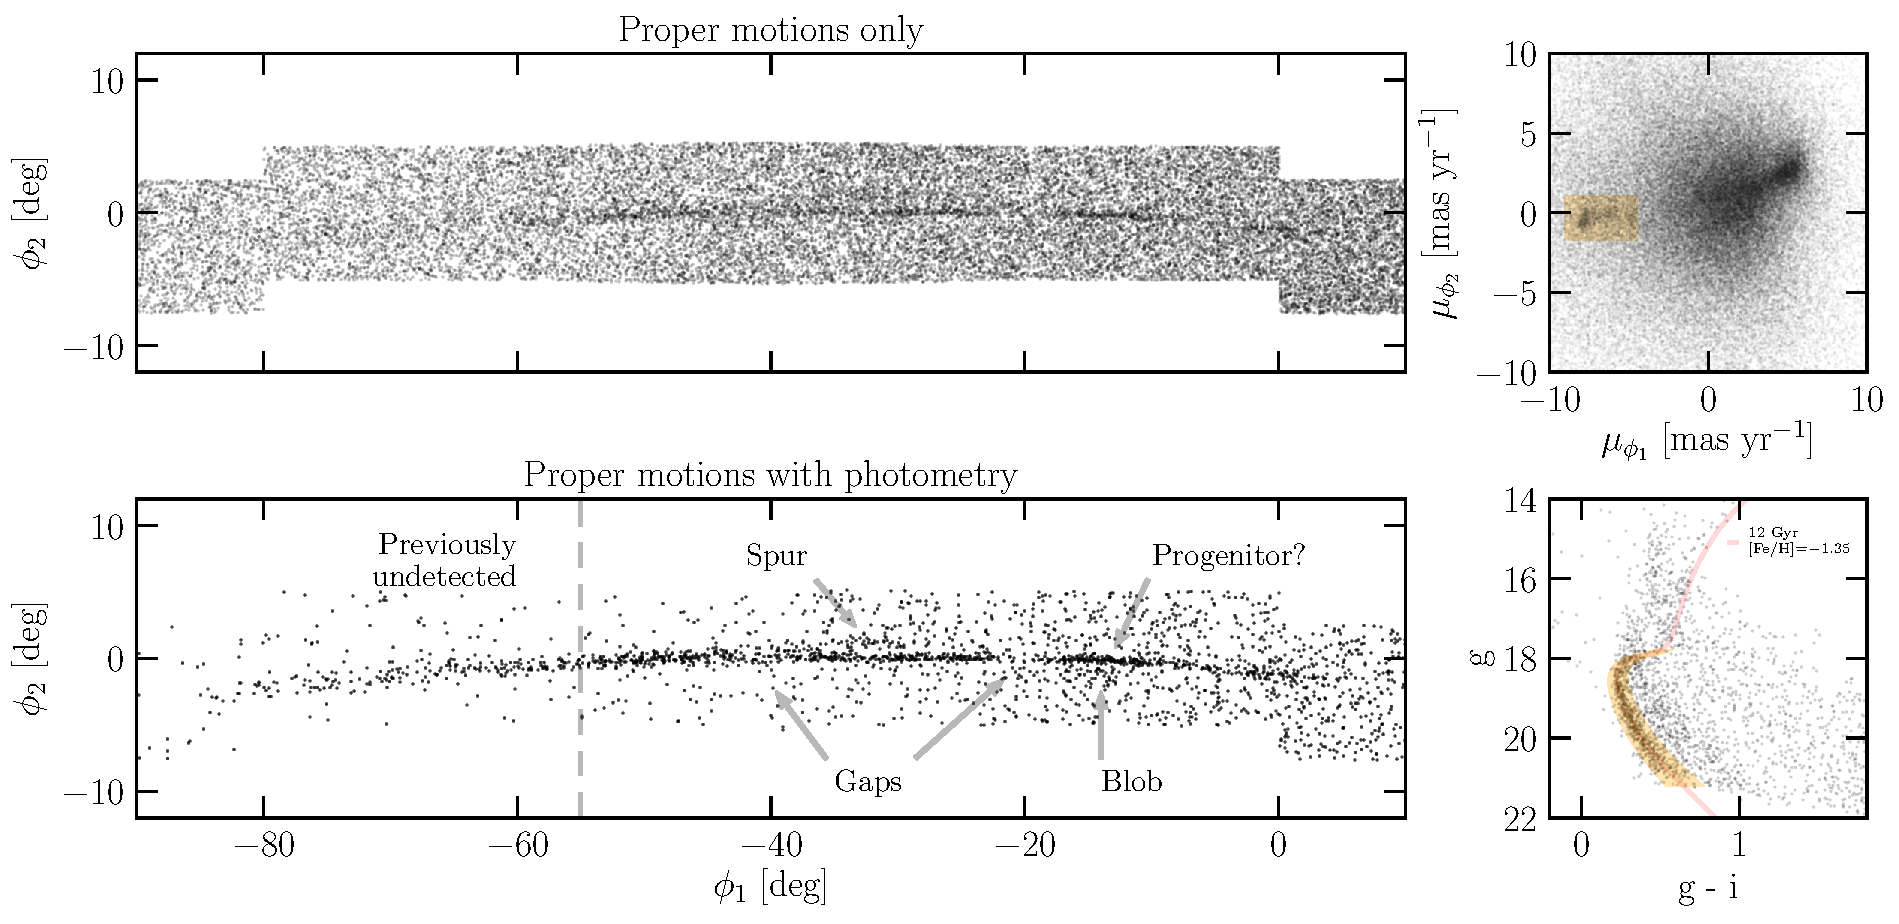
\includegraphics[width=\textwidth]{gd1_sample.pdf}
\end{center}
\caption{
On-sky positions of likely GD-1 members, in the coordinate system aligned with the stream.
GD-1 is apparent as an overdensity in retrograde proper motions (orange box on the top right panel), so a proper motion selection already reveals the stream in positions of individual stars (top left).
The stream population is older and more metal poor than the field Milky Way population, so the stream also stands out in the color-magnitude diagram (bottom right).
Additional photometric selection of the stream's main sequence (orange region in the CMD) unveils the stream in unprecedented detail (bottom left).
This map extends the stream by $20^\circ$, identifies a plausible location of the progenitor at $\phi_1\sim13^\circ$, confirms the existence of a significant gap at $\phi_1\sim-20^\circ$, shows additional under-densities at $\phi_1\sim-40^\circ,-5^\circ$ and for the first time finds stream overdensities off from the main track of a cold stream at $(\phi_1,\phi_2)\sim(-35^\circ,-1^\circ)$ and $(-15^\circ,-2^\circ)$.
}
\label{fig:selection}
\end{figure}

To improve the contrast of the stream over the background, we cross-match the
sample to the \pans\ photometric catalog and use the photometry to further clean
the sample.
\figurename~\ref{fig:selection} (bottom right) shows the distribution of
proper-motion-selected candidate stream stars within $\left|\phi_2\right| <
1^\circ$ in a \pans\ color-magnitude diagram (CMD) de-reddened following \citet{Schlafly:2011}.
The over-plotted isochrone (red line) is from the MESA Isochrones \& Stellar
Tracks (MIST; \citealt{Dotter:2016, Choi:2016, Paxton:2011}) and represents a
$12~\textrm{Gyr}$ old population with $\feh = -1.35$ at a distance of
$7.8~\kpc$.
We use this isochrone to motivate a polygonal selection in de-reddened $g-i$
color and apparent $g$-band magnitude, as visualized by the shaded region in the
bottom right panel of \figurename~\ref{fig:selection}.

\figurename~\ref{fig:selection} (bottom left) shows the final sample of GD-1
stream member candidates after selecting on both proper motion and photometry.
The GD-1 stream is clearly visible in the point density of \emph{individual} stars (the
positions are not binned); this is the most pure view of the stream to date.
The increased contrast shows that the stream extends at least another $20^\circ$
to negative longitudes.
Furthermore, the stream reaches its highest surface density where it is the narrowest ($\phi_1\sim-13^\circ$), so this map might have uncovered the location of its elusive progenitor.
Several of the under-densities and gaps hinted at from photometric selection
alone (\citealt{Koposov:2010, Carlberg:2013}) appear as striking features in
this significantly cleaner map of the GD-1 stream.
Finally, at least two new features are visible in this new view of the stream:
(1) ``the spur,'' stars above the main stream track (in $\phi_2$) between
$-40^\circ \lesssim \phi_1 \lesssim -30^\circ$, and (2) ``the blob,'' stars
below the main stream track between $-20^\circ \lesssim \phi_1 \lesssim
-10^\circ$.
We discuss each of these in more detail in \sectionname
s~\ref{sec:results}--\ref{sec:discussion} below.


\section{Results}
\label{sec:results}

We extract high-confidence stream stars from the proper motion and CMD selected
sample by further selecting stars close to the main stream track.
We use these main stream track stars to study the global properties of the
stream (\S\,\ref{sec:res_global}), and find interesting substructures off of the main stream track (\S\,\ref{sec:res_gap}).

\subsection{Global properties}
\label{sec:res_global}

To study the global properties of the stream as a function of stream longitude,
we extract stream stars around a low-order polynomial model for the median
stream latitude, $\phi_2$, as a function of stream longitude, $\phi_1$.
In detail, we find stream ridge points by computing a running median in $\phi_2$
in steps of $2^\circ$ with a window size of $4^\circ$ along $\phi_1$, then fit a
second-order polynomial to the ridge points to find $\phi_{2,
\textrm{track}}(\phi_1)$.
We define the stream as the region within $\left| \phi_2 - \phi_{2,
\textrm{track}}(\phi_1) \right| < 0.75^\circ$.
\figurename~\ref{fig:track-and-model} (top panel) again shows the
high-confidence stream stars, and the two curved lines (blue) show the adopted
upper and lower boundary of the stream region.

We extract properties of the stream from the region defined above as a function
of $\phi_1$ by computing stream properties in overlapping windows:
we set the window size to $4^\circ$ in $\phi_1$, and shift the window center by
$1^\circ$ in longitude for each measurement.
Rows 2--5 in \figurename~\ref{fig:track-and-model} show the background-subtracted
stream surface density, \todo{$\Sigma$?}, the median latitude, $\phi_2$, and median proper motions,
$\mu_{\phi_1}$ and $\mu_{\phi_2}$, extracted in this way, and the associated empirical scatters
(blue lines and shaded regions).
We estimate the local background surface density as an average of areas north and south from the bounded stream region.

\begin{figure}
\begin{center}
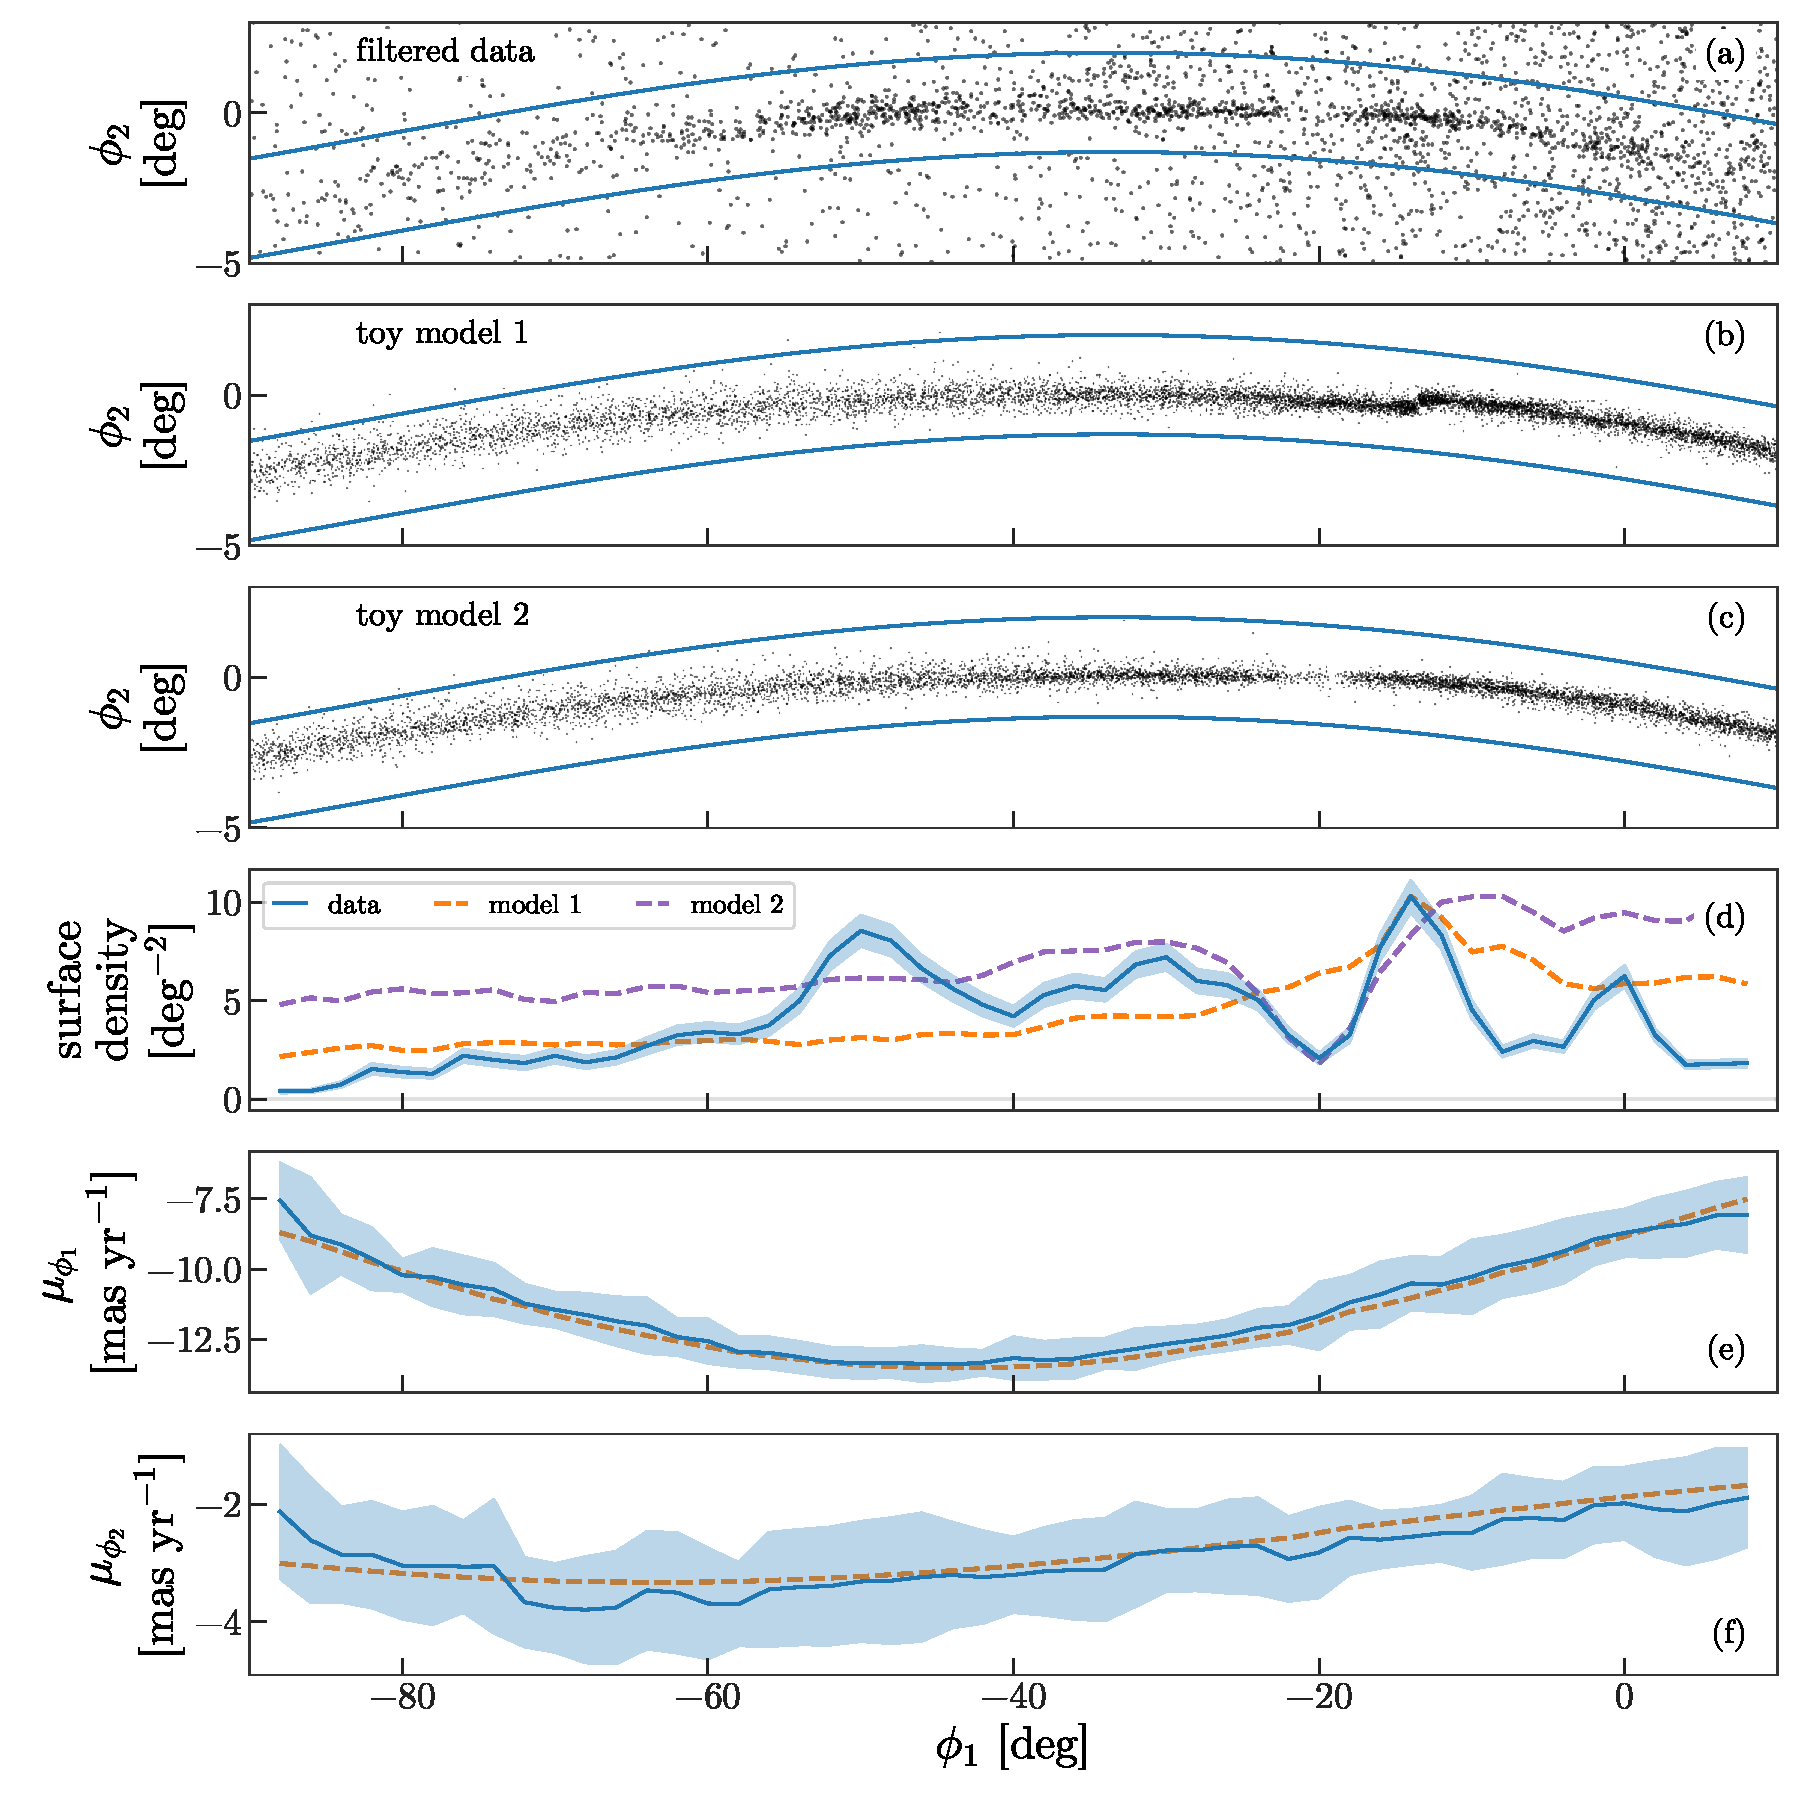
\includegraphics[width=\textwidth]{track_observables.pdf}
\end{center}
\caption{%
\todo{APW}
}
\label{fig:track-and-model}
\end{figure}

Clear density variations, also apparent in the 2D positions of the sources,
manifest as sharp features in the surface density estimates along the stream.
These are not a result of variable dust extinction or completeness variations
from the \gaia\ scanning pattern.
First, the visible portions of the GD-1 stream are located at high Galactic
latitudes ($b > 20^\circ$), and we therefore do not expect significant dust
extinction or variations in extinction within the stream region.
For stream longitudes $-60^\circ < \phi_1 < 10^\circ$ and $-1^\circ < \phi_2 <
1^\circ$, the median $V$-band extinction is $\textrm{med}\left(A_V\right) =
0.04~\textrm{mag}$, and the dispersion in $A_V$ in this region is $\sigma_{A_V}
\approx 0.03~\textrm{mag}$, as computed from the SFD
extinction map (\citealt{Schlegel:1998}).
For longitudes $\phi_1 < -60^\circ$, as the stream approaches the Galactic disk,
dust extinction becomes more appreciable, and the stream stars are harder to
select apart from the background.
Second, each star in our sample has at least XX visibility periods, while the sample median and variance are XX and XX, respectively, guaranteeing a robust estimate of proper motions.
Variations in the number density of faint stars originating from the scanning pattern are XX times smaller than the density variations in the stream, and their spatial distribution does not map to the stream features.
% The relative ratios between different over- and under-densities might be affected by the \gaia\ completeness at the faint end, but they 
\todo{check above sentences +  fill in}

The density variations likely represent real morphological changes along the
GD-1 stream, as have been suggested before from binned samples of
color-magnitude-selected GD-1 stars (\citealt{Carlberg:2013, DeBoer:2018}).
The deep under-densities we see from the kinematically-cleaned sample correspond
to previously reported gaps in the stream.
There is also a well-defined, sharp over-density in the surface density profile
close to $\phi_1 \approx -13^\circ$ with roughly symmetric under-densities on
either side:
this is suggestive of a progenitor system in the final stages of dissolution
(\todo{cite who}).
% \todo{Table of locations, sizes, and density constrasts for the features?}

We compare the measured stream properties to a simple model for the phase-space
density of the stream, generated by only simulating the orbital evolution of
cluster stars once they are tidally stripped from the progenitor.
In detail, during simulation, star particles are released from the Lagrange
points of the cluster with a spread in position and velocity set by the mass of
the satellite and the location within the host galaxy, with some tunable scale
parameters.
We use the parametrization and adopted scale parameters of \citet{Fardal:2015},
who fit the release distribution parameters by comparing to full $N$-body
simulations across a range of mass and orbital parameters.
This method can accurately reproduce the mean track of the resulting stream, but
the density of stars along the stream depends strongly on the mass-loss history
and internal kinematics of the progenitor system.
Here we assume a constant mass-loss rate, and release stream particles uniformly
in time from each Lagrange point; these choices match results from more detailed numerical experiments of globular cluster disruption \citep[e.g.,][]{Kupper:2012}.

To compute initial conditions for the stream model, we fit an orbit to the
observed properties of the stream in a fixed model for the gravitational
potential of the Milky Way.
We use a three-component potential model to represent the Galaxy, consisting of
a disk (\citealt{Miyamoto:1975}), a bulge
(\citealt{Hernquist:1990}), and a spherical dark matter halo
(\citealt{Navarro:1996}).
We set the disk scale-length parameters to closely match the disk model found in
\citet{Bovy:2015}, and other parameters are set to reproduce an approximately
flat rotation curve between $5 < R < 15~\kpc$ with a circular velocity at the
solar circle, $v_{\textrm{circ}, \odot} \approx 230~\kms$.

\begin{figure}
\begin{center}
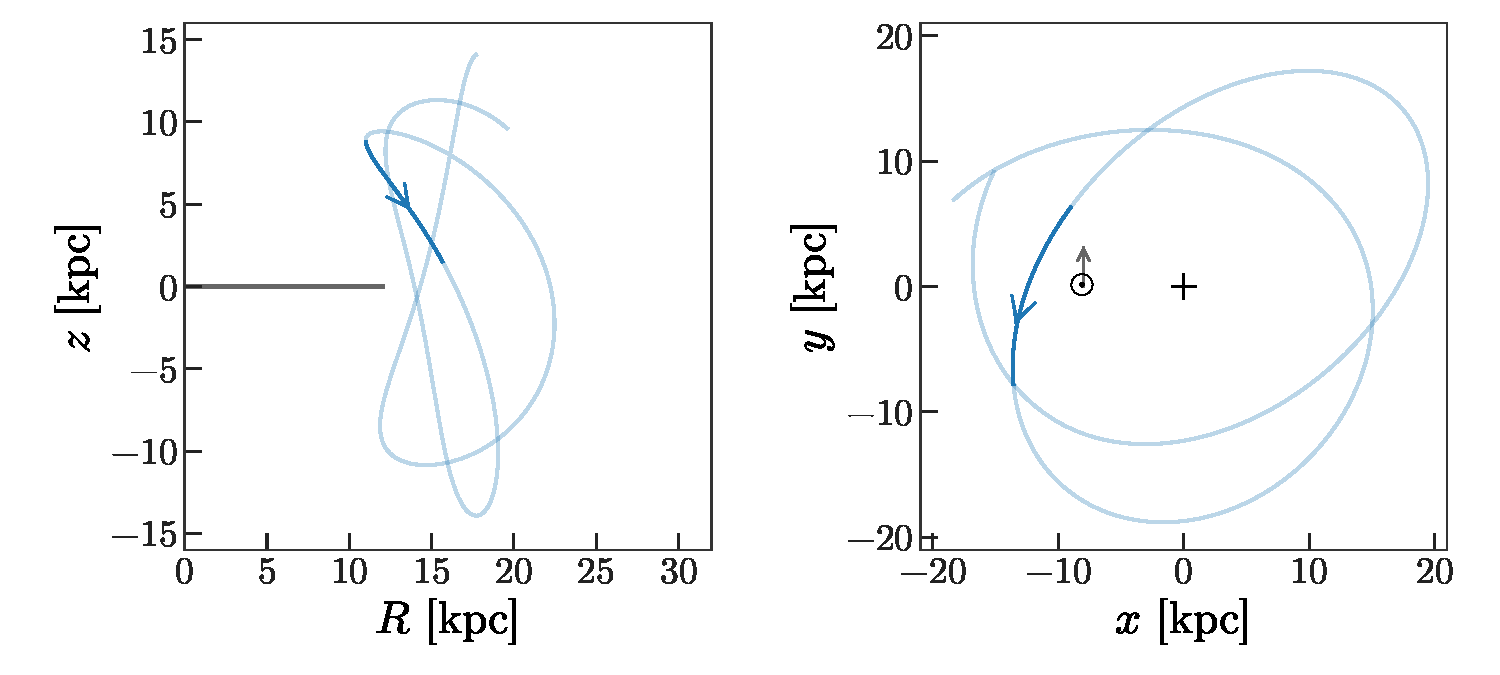
\includegraphics[width=\textwidth]{orbitfit.pdf}
\end{center}
\caption{%
\todo{APW}
}
\label{fig:orbitfit}
\end{figure}

To initialize the model stream generation, we assume that the present day (i.e.
final) position of the progenitor system is at $\phi_1 = -13.5^\circ$, the peak
of the observed surface density profile.
We integrate backwards for $4~\textrm{Gyr}$ using the orbital parameters at this
location using the Leapfrog integration scheme with a timestep of
$0.5~\textrm{Myr}$, then begin the model stream generation using the Lagrange
point stripping method discussed above.
Stream particles are release at each timestep of the progenitor orbit
integration, resulting in 16,000 stream particles by the end of the model stream
generation.
We assume an initial progenitor mass of $M=10^5~\msun$, and linearly decrease
the mass of the progenitor until present day, where we assume $M = 0~\msun$
(i.e. fully disrupted).
Stream properties computed from this resulting model stream are plotted in
\figurename~\ref{fig:track-and-model} as \todo{XX}.

\figurename~\ref{fig:orbitfit} shows \todo{APW: ...}


\subsection{Off-track features}
\label{sec:res_gap}

- overdensities apparent beyond the main stream track used in previous section -- if truly associated with the stream, this would be a novel insight into disruption from the \gaia\ mission
- since some contamination still remains present, it is possible that this is a variation in the MW population, just randomly coming into our selection boxes
- we thus perform an experiment and compare cmd and proper motions of spur and blob fields to stream and background fields to see which they are associated with

\begin{figure}
\begin{center}
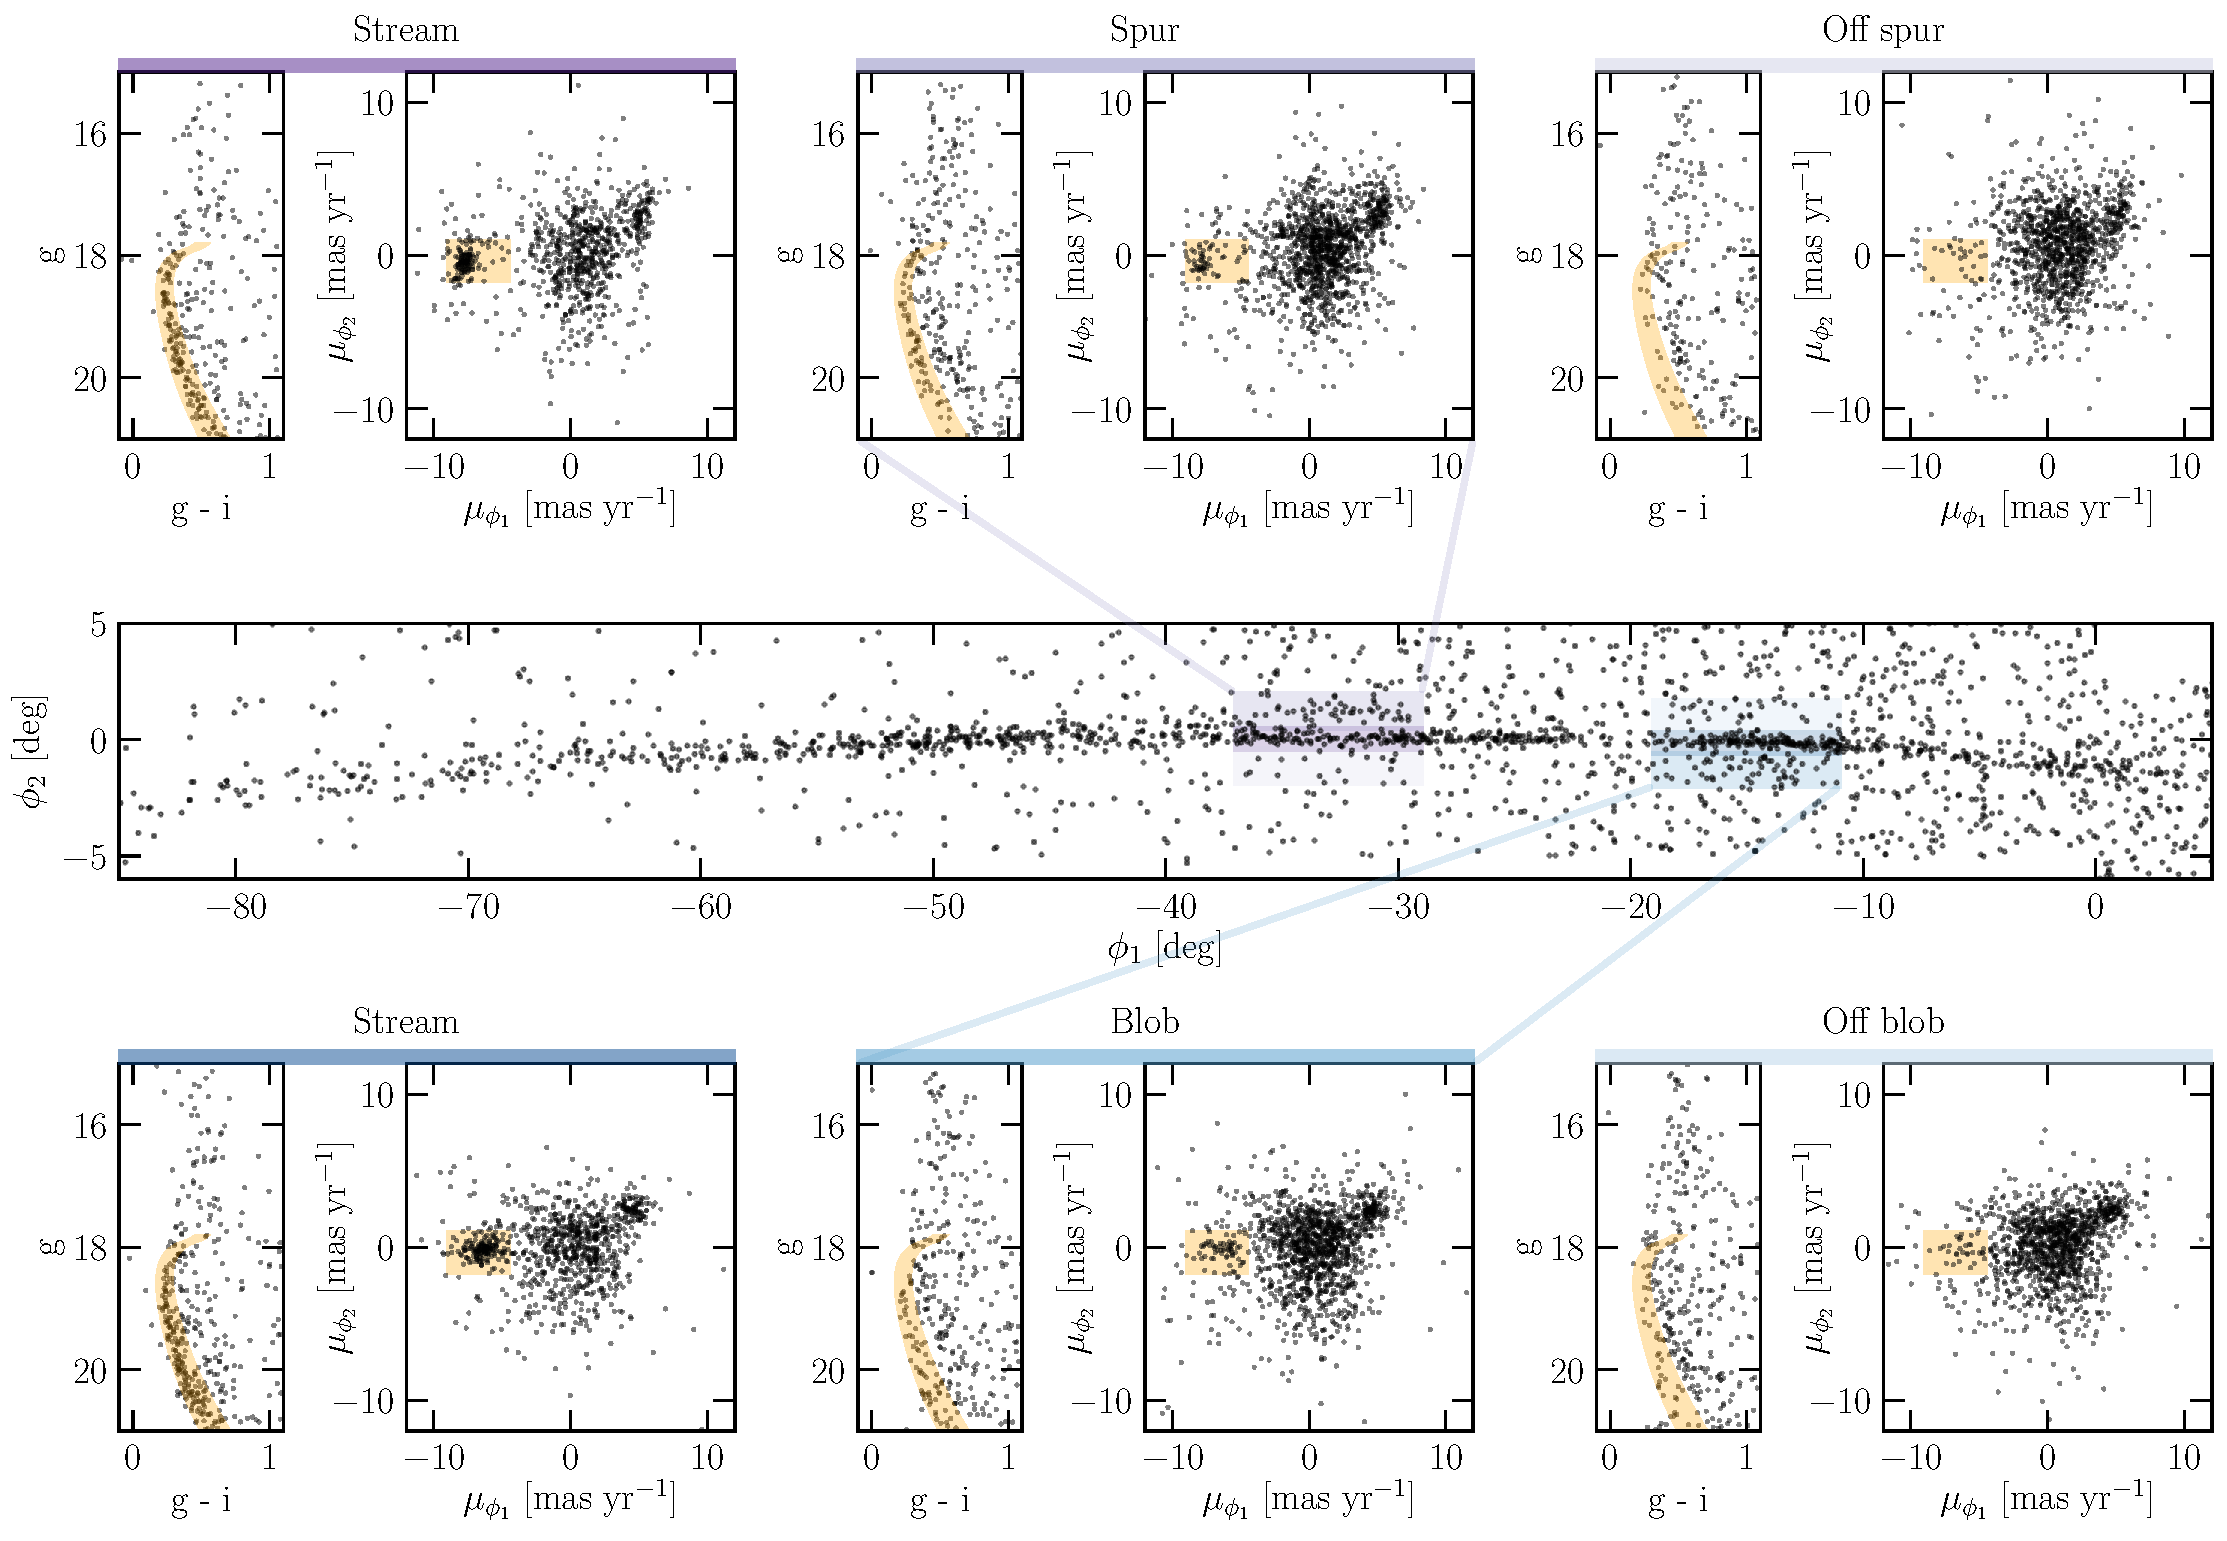
\includegraphics[width=\textwidth]{features.pdf}
\end{center}
\caption{
Color-magnitude and proper-motion diagrams of fields associated with a spur above GD-1 (top), and fields related to the blob below GD-1 (bottom).
The left-most pair of panels show properties in stream fields (darkest rectangles in the middle panel), the middle pairs present spur and blob (medium rectangles), while the right-most panels have fields on the opposite side from spur and blob (lightest rectangles).
Selection boxes used to select stars shown in the middle panel are shown in orange in all CMD and proper-motion panels.
Both the spur and the blob fields have more stars in the CMD selection box than the corresponding control fields.
Proper motions of these stars follow the distribution of stars in adjacent stream fields, thus confirming the association of these off-track features with GD-1.
}
\label{fig:features}
\end{figure}

- central panel of figure~\ref{fig:features} shows the map of GD-1, with fields of interest in shaded rectangles
- we first analyze the spur, region, stream same phi1, phi2 below, and an off-stream field in phi2
- for each of these fields, we show a pair of plots in the top row: cmd on the left and proper motions on the right. 
- we first select on pm, and show cmd, and then select on cmd and show pm
- in both of these spaces, selection regions used to make the main catalog are shown in shaded orange.
- stream field (top left) has clear overdensity in the cmd selection box and clusters in proper motion
- on the other hand, the off field has some stars entering both selection boxes, but without any overdensities in either
- the spur field has fewer stars than the stream, but XX more than expected from the MW alone
- furthermore, the distribution in selection boxes is distributed similarly as in the stream field
- this confirms the association, but we note that in detail they differ
- median in pm offset from the stream field just below is XX, YY mas yr
- also dispersion different
- don't have enough stars to measure distance from the turn-off, so defer to future studies to measure by some other means, e.g., from photometry

- analogous paragraph for blob on the bottom

% - Spur vs. blob
% - Estimate velocity offset and significance
% - No indication of these features in previous work

% \figurename~\ref{fig:features} (middle panel) again shows the proper-motion and CMD selected stream stars, with interesting features

\section{Discussion}
\label{sec:discussion}

- novel way to identify members -- helpful that retrograde, but hopefully also applicable to other streams as kinematic important
- gd-1 even longer -- useful for potential constraints --> future

- progenitor? if confirmed, can create more realistic models (so far only modeled the whole stream as just a leading or trailing arm)
- to confirm -- measure actions, which change direction (some bovy paper)?

- no longer simple stream, discuss possible causes
- evaporation?

- spur \& blob as related to gaps? -- classify possible explanations in this way
- if from encounter -- could get more info on the perturber than from the gaps alone, say from delta v

- progenitor
-- rotation -- could explain spurs, but not gaps?

- smooth component of the potential?
-- show orbit
-- chaos?
-- \todo{APW} bar -- hard to make small feature, size should be ~angular size of the bar at stream (influence of bar should be a radian of the stream) + relative velocity (retrograde)

- encounters?
-- work out mass / time combinations in impulse approximation
-- comment on GMC vs subhalo

- future:
-- radial velocities, measure 3d velocity structure (unique predictions)
- delta energy, 
- cleaner selection (any stars in the gap)

- (should go at least to symmetric in positive), not captured with naive selection, as there are gradients
- prediction: very negative rv, should be easy to map the full extent 

% -- tests for other outstanding issues
-- model facets of stream morphology to ascertain if consistent with encounter signatures
-- so far a lot of focus on gaps produced in encounters -- extra features we detected beside the GD-1 track suggest that further theoretical focus on scattered material is needed to fully understand its dynamical history


% \section{Conclusions}
% \label{sec:conclusions}

% From the combined proper motion and CMD selection of stream members
% (\sectionname~\ref{sec:data}), it is now clear that the GD-1 stream extends
% at least $90^\circ$ in apparent length.
% Several clear under-densities and gaps are also
% \figurename~\ref{fig:sfd-cmd} (middle panel) again shows the proper-motion and CMD selected stream stars, with several features


\acknowledgements{
It is a pleasure to thank
Vasily Belokurov,
Andrew R. Casey,
Marla Geha,
David W. Hogg,
Benjamin D. Johnson,
Kathryn V. Johnston,
Sergey Koposov,
Mariangela Lisanti,
Edward Schlafly,
and David N. Spergel for useful discussions and feedback.

This work has made use of data from the European Space Agency (ESA) mission {\it
Gaia} (\url{https://www.cosmos.esa.int/gaia}), processed by the {\it Gaia} Data
Processing and Analysis Consortium (DPAC,
\url{https://www.cosmos.esa.int/web/gaia/dpac/consortium}). Funding for the DPAC
has been provided by national institutions, in particular the institutions
participating in the {\it Gaia} Multilateral Agreement.  This research was
started at the NYC Gaia DR2 Workshop at the Center for Computational
Astrophysics of the Flatiron Institute in 2018 April.

AB acknowledges generous support from the Institute for Theory and Computation
at Harvard University.
All code used in this work and all results are available at
\url{https://github.com/adrn/GD1-DR2}.
}

\software{
    \package{Astropy} \citep{astropy},
    \package{dustmaps}\footnote{\url{https://github.com/gregreen/dustmaps}},
    \package{gala} \citep{gala},
    \package{IPython} \citep{ipython},
    \package{matplotlib} \citep{mpl},
    \package{numpy} \citep{numpy},
    \package{scipy} \citep{scipy}
}

\bibliographystyle{aasjournal}
\bibliography{gd1}

\clearpage

% \appendix
% \section{Completeness and the \gaia\ scanning pattern}
% \label{sec:completeness}

% \figurename~\ref{fig:XX} (XX panel) shows the $V$-band extinction
% in the region around the GD-1 stream, computed from the
% Schlegel-Finkbeiner-Davis extinction map (\cite{Schlegel:1998}; hereafter SFD).

% % Notebook:
% \begin{figure}[h]
% \begin{center}
% \includegraphics[width=0.7\textwidth]{nvisits.pdf}
% \end{center}
% \caption{%
% TODO
% \label{fig:TODO}
% }
% \end{figure}


\end{document}
